\documentclass[a4paper]{article}

%% Language and font encodings
\usepackage[french]{babel}
\usepackage[utf8x]{inputenc}
\usepackage[T1]{fontenc}


%% Sets page size and margins
\usepackage[a4paper,top=3cm,bottom=2cm,left=3cm,right=3cm,marginparwidth=1.75cm]{geometry}

%% Useful packages
\usepackage{amsmath,amsfonts,amssymb,amsthm,epsfig,epstopdf,titling,url,array}
\usepackage{graphicx}
\usepackage[colorinlistoftodos]{todonotes}
\usepackage[colorlinks=true, allcolors=blue]{hyperref}
\usepackage{comment}
\theoremstyle{plain}
\newtheorem{thm}{Théoreme}[section]
\newtheorem{lem}[thm]{Lemme}
\newtheorem{prop}[thm]{Proposition}
\newtheorem*{cor}{Corollary}
\theoremstyle{definition}
\newtheorem{nota}{Notation}[section]
\newtheorem{defn}{Définition}[section]
\newtheorem{conj}{Conjecture}[section]
\newtheorem{exmp}{Exemple}[section]
%\theoremstyle{proof}
\newtheorem{dem}{Démonstration}
\theoremstyle{remark}
\newtheorem*{rem}{Remark}
\newtheorem*{note}{Note}

\usepackage{cellspace}
\usepackage{diagbox}

\begin{document}
\begin{titlepage}
  \begin{sffamily}
	\begin{center}
	
		\textsc{\Large Rapport de Projet Maths Info 2019}\\
		\vspace{9.5cm}
		{ \huge  Le modèle SIR, modélisation des épidémies\\[0.4cm] }
		
		\vspace{10cm}
		% Author and supervisor
		\begin{minipage}{0.4\textwidth}
			\begin{flushleft} \large
				\textsc{Bétend Marie}\\
				\textsc{Caye Flore}\\
			\end{flushleft}
		\end{minipage}
		\begin{minipage}{0.4\textwidth}
			\begin{flushright} \large
				\textsc{Superviseur : M.Alessandro Zilio}
			\end{flushright}
		\end{minipage}
		
		\vfill
		
		% Bottom of the page
		{\large 	Mars-Juin 2019}
		
	\end{center}
\end{sffamily}
\end{titlepage}
\tableofcontents
\newpage
\section{Introduction}

Ce document à été écrit dans le cadre du projet Maths-informatique de notre 3ème année de licence.

Nous avons étudié une modélisation de la diffusion d'une maladie, pour étudier sa propagation au sein d'une population, et déterminer les conditions menant à une épidémie.
Les épidémies sont en effet un phénomène assez intriguant, nous avons tous entendu parler des mouvements de peste au moyen âge, notamment l'épisode de la peste noire qui a décimée 60\% de la population européenne %verifier qu'il s'agit du bon nom.

Nous présenterons dans ce rapport un modèle simplifié de la propagation d'une maladie, en étudiant l'évolution de la population au cours du temps. Nous étudierons  également les déplacements de populations, à l'aide de graphes, sur des réseaux de transports. Enfin, en regroupant nos deux modèles, nous essayerons de simuler la propagation de l'infection  dans une population en mouvement.




\section{Modélisation d'une épidémie via le modele SIR}
\subsection{Origine}
Le modèle SIR a été présenté par W.O.Kermack et A.G.McKendrick à Londres et Cambridge en 1927. Avec ce modèle, les deux scientifiques ont étudiés l’évolution de l’épidémie de peste à Bombay, survenue en 1905-1906.
C'est un modèle classique en épidémiologie, car malgré sa simplicité, il nous permet de tirer des conclusions intéressantes.

\subsection{Qu'est ce que le modèle SIR}
%Petit point historique de qui quoi pourquoi comment, 


Nous souhaitons étudier la propagation d'une maladie au sein d'une population, afin de comprendre quels sont les paramètres et les mécanismes à l'origine d'une épidémie. Pour ce faire, nous allons considérer une situation idéalisée, mais qui va nous permettre de constater des faits intéressants.

Imaginons que la population que l'on observe soit constante; on va diviser cette population en trois groupes : les individus Sains et susceptibles d'être inféctés par une maladie, les individus Infectés et les individus Remis de la maladie (guéris en d'autres termes). Ici nous allons supposer que les individus Remis de la maladie ne peuvent plus être infectés, ils ont par exemple développé une immunité contre l'infection ou bien ils sont décédés et ne peuvent donc plus tomber malade. Nous n'allons pas non plus considérer le temps d'incubation de la maladie : un individu sain devient immédiatement infecté lorque qu'il contracte la maladie et peut transmettre a son tour l'infection, sans phase intermédiaire. 

Ce modèle est appelé le modèle SIR.

\begin{figure}[!h]
\begin{center}
   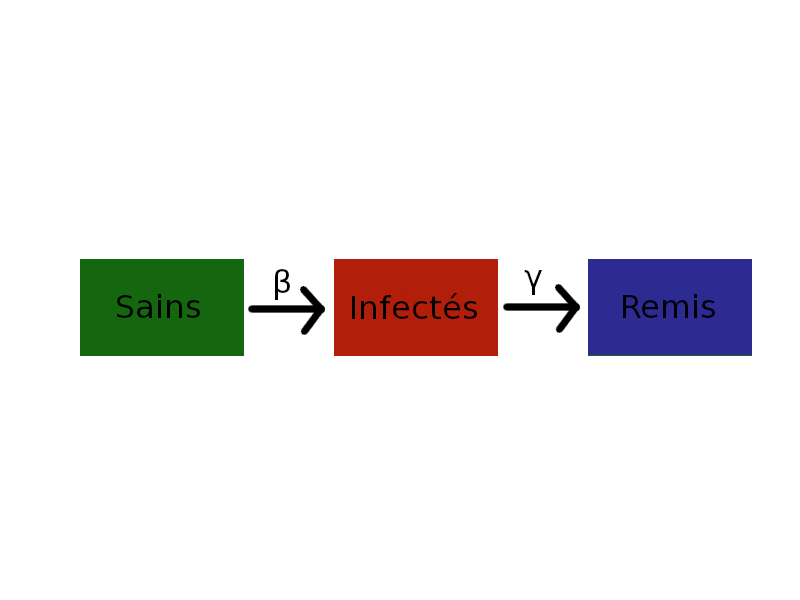
\includegraphics[scale= 1.2]{SIR.png}
   \end{center}
     \caption{Le modèle SIR}
\end{figure}

Par la suite nous utiliserons les notations suivantes : $N$ pour le nombre d'indivdus total de la population, $S$ pour les individus sains, $I$ les infectés et $R$ les remis.
Comme la population est supposée constante, à tout instant on a : $ N = S + I + R$.

Ces populations évoluent au cours du temps.
On peut modéliser cette évolution par des fonctions réelles de la variable $t \geq 0$, ce qui nous donne les équations différentielles suivantes :
\begin{align}
\label{dS}
&\frac{dS}{dt} = -\beta\frac{SI}{N} \\
\label{dI}
&\frac{dI}{dt} = \beta\frac{SI}{N} - \gamma I \\
\label{dR}  
&\frac{dR}{dt} = \gamma I 
\end{align}

Nous allons surtout nous intérésser à \eqref{dS} et \eqref{dI}. En effet \eqref{dR} est redondante car
\begin{align*}
\frac{d}{dt} (S + I + R) = \frac{dN}{dt}
\end{align*} 
et comme N est constante, on a
\begin{align*}
\frac{d}{dt}(S + I +R) = 0 .
\end{align*}
On a donc besoin seulement de 2 équations.

Expliquons maintenant d'où nous viennent ces formules.
Pour \eqref{dR}, on considère que le nombre de guérisons est proportionnel au nombre de personnes infectés, d'où une augmentation dans le temps d'un coefficient $\gamma$. Logiquement la guérison d'individus infectés diminue cette population ci, d'ou le terme $-\gamma I$ dans \eqref{dI}.

Pour \eqref{dS}, la population saine subit $C$, la contagion sur un intervalle de temps $\Delta t$; c'est à dire 
\begin{center}
$S(t+\Delta t) = S(t) + C(t + \Delta t)$
\end{center}
Cette contagion est proportionnelle à la probabilité qu'un individu sain rencontre un individu infecté, on a donc 
\begin{center}
$C(t, \Delta t) \approx \alpha P_{SI}(t, \Delta t)$
\end{center}

Maintenant supposons que l'on divise le territoire de la population en M cases. Supposons également que la probablité qu'un individu sain se trouve dans une case est $\frac{S}{M}$, et celle d'avoir un individu infécté est $\frac{I}{M}$. Ces deux variables suivent une loi binomiales, de paramètres (S , $\frac{1}{M}$) et (I , $\frac{1}{M}$). Elles sont de plus indépendants.

\begin{align*}
P_{SI}(t, \Delta t) &= P(\text{"il y a au moins un individu sain et un individu infecté sur une case"})\Delta t \\
&=[1 - P(\text {"il n'y a pas d'individu sain sur une case"} \cup \text{"il n'y a pas d'individus infectés sur une case"})]\Delta t \\
&=[1 - [P(\text{"il n'y a pas d'individu sain sur une case"})P(\text{"il n'y a pas d'individus infectés sur une case"})\\
&  - P(\text {"il n'y a pas d'individu sain sur une case"} \cap \text{"il n'y a pas d'individus infectés sur une case"}]]\Delta t \\
&=[1 - [(1 - \frac{1}{M})^S + (1 - \frac{1}{M})^I - (1 - \frac{1}{M})^S(1 - \frac{1}{M})^I]]\Delta t \\
\end{align*}

Par la formule du binôme de Newton  
\begin{align*}
P_{SI}(t, \Delta t) &=[1 - [\sum_{k=0}^{S} \binom{S}{k}1^k (\frac{-1}{M})^{S-k}  + \sum_{k=0}^{I} \binom{I}{k}1^k (\frac{-1}{M})^{I-k} - \sum_{k=0}^{S} \binom{S}{k}1^k (\frac{-1}{M})^{S-k}\sum_{k=0}^{I} \binom{I}{k}1^k (\frac{-1}{M})^{I-k}]]\Delta t \\
&= [1 - [\sum_{k=0}^{S} \frac{S!}{k!(S-k)!} (\frac{-1}{M})^{S-k}  + \sum_{k=0}^{I} \frac{I!}{k!(I-k)!} (\frac{-1}{M})^{I-k} - \sum_{k=0}^{S} \frac{S!}{k!(S-k)!} (\frac{-1}{M})^{S-k}\sum_{k=0}^{I} \frac{I!}{k!(I-k)!} (\frac{-1}{M})^{I-k}]]\Delta t \\
\end{align*}

Pour N suffisamment grand, on a le développement à l'ordre 2 suivant :
\begin{align*}
P_{SI}(t, \Delta t) &=[1 - [1 + \frac{-S}{M}+\frac{S^2-S}{2M^2}+1+\frac{-I}{M}+\frac{I^2-I}{2M^2}-(1+\frac{-S}{M}+\frac{S^2-S}{2M^2})(1+\frac{-I}{M}+\frac{I^2-I}{2M^2})]]\Delta t \\
&= [1 - [1 + \frac{-S}{M}+\frac{S^2-S}{2M^2}+1+\frac{-I}{M}+\frac{I^2-I}{2M^2}-(1+\frac{-I}{M}+\frac{I^2-I}{2M^2} +\frac{-S}{M}+ \frac{SI}{M^2}+\frac{S^2-S}{2M^2} + o((\frac{-1}{M})^3))]]\Delta t \\
&= [1 - 1 + \frac{S}{M} - \frac{S^2-S}{2M^2} - 1+\frac{I}{M} - \frac{I^2-I}{2M^2} +1+\frac{-I}{M}+\frac{I^2-I}{2M^2} +\frac{-S}{M}+ \frac{SI}{M^2}+\frac{S^2-S}{2M^2} + o((\frac{-1}{M})^3)]\Delta t \\
&=[\frac{SI}{M^2} +o((\frac{-1}{M})^3)] \Delta t\\
\end{align*}

%Est ce que ca fait bcp de sens ? Verification au niveau des delta t a faire%
On en déduit finalement que la probabilité d'une contagion est proportionelle à $SI \Delta t$ : 
\begin{center}
    $C(t, \Delta t) \approx \alpha SIk \Delta t +  o(\Delta t)$
\end{center}
En posant $\alpha k = \frac{- \beta}{N}$ et en remplaçant, on obtient : 
\begin{center}
    $S(t+\Delta t) = S(t) + \frac{- \beta}{N}SI\Delta t + o(\Delta t)$
\end{center}
En supposant que $S$ est une fonction régulière, on a le développement de Taylor suivant :
\begin{align*}
    &S(t + \Delta t) =  S(t) + \Delta t  S^{'}(t)+o(\Delta t)\\
    \Leftrightarrow &S(t) + \Delta t S^{'}(t) + o(\Delta t)= S(t) + \frac{- \beta}{N}SI\Delta t + o(\Delta t)\\
    \Leftrightarrow &S^{'}(t) = \frac{- \beta}{N}SI + o(1)\\
    \Leftrightarrow &S^{'}(t) = \frac{- \beta}{N}SI 
\end{align*}
    


\subsection{Simplification en un système équivalent}
Le système d'équations 

\begin{align*}
\frac{dS}{dt}&= -\beta\frac{SI}{N} \\
\frac{dI}{dt}&= \beta\frac{SI}{N} - \gamma I \\
\frac{dR}{dt}&= \gamma I
\end{align*}

décrit l'évolution des différentes catégories de population (Sains, Infectés, Remis) en fonction du temps. Pour simplifier, nous allons étudier non plus le nombre d'individus de chaque catégories, mais la proportion de chacun des groupes. On considère alors (s(t), i(t), r(t)) telles que
\begin{align*}
s(t)&=\frac{S(t)}{N}\\
i(t)&=\frac{I(t)}{N}\\
r(t)&=\frac{R(t)}{N}
\end{align*}
On se passe à nouveau de $R(t)$ et $r(t)$ car elles sont redondantes dans leurs systèmes d'équations différentielles respectifs. 
Le système d'équations différentielles en $s$, et $i$ est alors:

\begin{align}
    \label{cauchy1}
    s'(t)&= - \beta s(t)i(t) \\
    \label{cauchy2}
    i'(t)&= \beta s(t)i(t) - \gamma i(t) \\
    \label{cauchy3}
    s(0)&= s_{0} \\
    \label{cauchy4}
    i(0)&= i_{0} 
\end{align}

Où $s_0, i_0 $ sont les valeurs initiales, définies de manière à ce que le problème de Cauchy admette une unique solution globale sur $\mathbb{R}^+$.
C'est ce problème de Cauchy que nous étudierons par la suite.
\subsection{Existence des solutions}
	\subsubsection{Outils pour le traitement des équations différentielles}
	On pose $f:U\subset\mathbb{R}^{n+1}\rightarrow\mathbb{R}^n$, définie sur l'ensemble produit $U=J\times\Omega$.
\begin{prop}
	Soit $f\in C^1(U, \mathbb{R}^n)$ avec $U\subset\mathbb{R}\times\mathbb{R}^n$. Alors $f$ est localement Lipschitzienne par rapport à la deuxième variable dans $U$.
\end{prop}
\begin{thm}[Théorème de Cauchy-Lipschitz]
\label{CL}
Soit $U\subset\mathbb{R}\times\mathbb{R}^n$ ouvert et $f: U\rightarrow \mathbb{R}^n$ localement Lipschitzienne par rapport à la deuxième variable dans $U$ et $(t_0,x_0)\in\mathbb{R}\times\mathbb{R}^n$.\\ Alors il existe une unique solution maximale définie sur un intervalle non vide $I_{(t_0, x_0)}\subset\mathbb{R}$ qui contient $t_0$.
\end{thm}
\begin{thm}[Corollaire du théorème de sortie de compacts]
\label{compact}
 Si l'image d'une solution maximale $u: \left]t_-, t_+\right[\rightarrow\mathbb{R}^n$ est contenue dans un compact $K\subset\mathbb{R}^n$ pour tout $t\in\left[t_0, t_+\right[$, alors $t_+=sup(J)$.
\end{thm}
\subsubsection{Intervalle relatif}
    Pour rappel, le modèle SIR ne représente des épidémies que dans des populations constantes (donc sur un temps suffisamment court pour ne pas considérer la démographie naturelle, et pour des maladies non mortelles). Ainsi la somme $S(t)+I(t)+R(T)=N$ est constante, ce qui implique $s(t)+i(t)+r(t)=1$ pour les proportions d'individus. De plus, $s, i$ et $r$ sont des parts de la populations, donc positives pour tout $t \geqslant 0 $. La fonction $r(t)$ ne servant qu'à équilibrer la somme, on a $0 \leqslant s(t)+i(t) \leqslant 1$. Il nous suffit alors d'étudier les solutions du système sur le triangle $T=\left\{(s,i) | s\geqslant0, i\geqslant0, s+i\leqslant1\right\}$. \\
    \subsubsection{Unicité de la solution}
	Posons
	\begin{equation}
	   \label{f}
	    f(t,s,i)=(- \beta s i, \beta s i - \gamma i)
	\end{equation}de $\mathbb{R}^{+}\times\mathbb{R}^{2+}$ dans $\mathbb{R}^{2+}$.
	On impose que $(s_0,i_0)$ appartiennent à $\mathbb{R}^{2+}$.
	$f$ est continûment dérivable sur $\mathbb{R}^{+}\times\mathbb{R}^{2+}$, donc $f$ est localement lipschitzienne en la deuxième variable uniformément en la première, et $(0,(s_0,i_0))$ appartient à $\mathbb{R}^{+}\times\mathbb{R}^{2+}$. On a réunis toutes les conditions pour appliquer le théorème de Cauchy-Lipschitz.\\
	Alors il existe une unique solution maximale $(s(t), i(t))$ définie sur un intervalle non vide $I_{max}\subset\mathbb{R}$ qui contient $0$.\\
	Il s'agit maintenant de déterminer cet intervalle $I_{max}$. En fait, par cohérence avec le modèle, il nous suffit d'étudier $I=I_{max}\cap\mathbb{R}^+$. On définit alors $t_{max}$ comme $I= \left[0,t_{max}\right[ $. Il nous reste à déterminer $t_{max}$. \newline
	On sait que $0 \leqslant s+i \leqslant 1$, donc $(s(t),i(t))\in \left[ 0,1 \right] ^2$ pour tout $t\in I_{max}$. Comme $\left[0,1\right]^2\subset\mathbb{R}^{2+}$ est un compact, on peut appliquer le théorème \hyperlink{compact}{de sortie de compact} avec $J=\mathbb{R}$. Ainsi $t_{max}=+\infty$.\\
	On considérera dans la suite $(s,i)$ la solution du problème de Cauchy (\eqref{cauchy1}, \eqref{cauchy2}, \eqref{cauchy3}, \eqref{cauchy4}) sur $\left[ 0, +\infty \right[$. Maintenant qu'on a prouvé l'existence et l'unicité d'une telle solution, on peut étudier le comportement relatif de $s$ et $i$ sur $T$.
	
    
  \subsection{Dépendance aux conditions initiales}
  \subsubsection{Allure générale}
    \begin{description}
    \item{$s:  $} $\beta$ est une constante positive (sinon la population saine augmente lorsqu'elle est infectée, et il y a une contradiction). $s(t)$ et $i(t)$ sont également positives ou nulles à tout temps t sur T. Donc $s'(t)= -\beta s(t)i(t)$ est négative. Ainsi, sur T, $s(t)$ est décroissante. %%schéma
    \item{$i:  $} Sur T, on considère $i'(t)=\beta s(t)i(t) -\gamma i(t)$. On cherche où s'annule $i'$ sur T. 
    \begin{align*}
    i'(t)=0 &\Leftrightarrow \beta s(t)i(t)=\gamma i(t)\\
    &\Leftrightarrow \beta s(t)=\gamma\\
    &\Leftrightarrow s(t)=\frac{\gamma}{\beta}
    \end{align*}
    %%schema
	\end{description}
 $i$ est donc croissante jusqu'en $t_{max}\in\mathbb{R}^+$ tel que $s(t_{max})=\frac{\gamma}{\beta}$ (quand $s$ atteint une telle valeur) puis $i$ est décroissante.\\
\subsubsection{Stabilité}
 	Soit $(s,0)$ un couple solution pour le problème de Cauchy.\\
 	C'est un équilibre pour le système, on a bien 
 	\begin{align*}
    s' &= 0\\
    i' &= 0
    \end{align*}
 	%%
 	Étudions la stabilité de ce point d'équilibre. Soit $J_f$ la matrice jacobienne de la fonction $f$ définie par \eqref{f}.
 	\begin{align}
 J_f\begin{pmatrix}
s\\ i\\
\end{pmatrix}
&=\begin{pmatrix}
-\beta i&-\beta s\\
\beta i&\beta s-\gamma\\
\end{pmatrix} 
\end{align}

Les valeurs propres de $ J_f\begin{pmatrix}
s\\ 0\\
\end{pmatrix}$ permettront de conclure quand à la stabilité de la solution en fonction des conditions initiales. 
L'évaluation en $(s,0)$ donne:
\begin{align}
J_f\begin{pmatrix}
s\\ 0\\
\end{pmatrix}
=\begin{pmatrix}
0&-\beta s\\
0&\beta s-\gamma\\
\end{pmatrix}
\end{align}
Les racines du polynôme caractéristique $p_{\lambda}$ associé à $ J_f\begin{pmatrix}
s\\ 0\\
\end{pmatrix}$, sont les valeurs propres de notre matrice.
\begin{align*}
p_{\lambda}&=det(J_f\begin{pmatrix}
s\\ 0\\
\end{pmatrix}-\lambda I_{2})\\
&=\begin{vmatrix}
-\lambda&-\beta s\\
0&\beta s-\gamma-\lambda\\
\end{vmatrix}\\
&=(-\lambda)(\beta s-\gamma-\lambda)\\
&=\lambda(-\beta s+\gamma+\lambda)\\
\end{align*}
Ainsi $\lambda=0$ ou $-\beta s+\gamma+\lambda=0 \Leftrightarrow\lambda=\beta s-\gamma$.

Un point d'équilibre est dit stable si les parties réelles des valeurs propres sont négatives ou nulles. Il est instable sinon. Étudions le signe de la valeur propre non-nulle en fonction de $s$.
\begin{align*}
\beta s-\gamma & \leqslant0\\
\Leftrightarrow s & \leqslant\frac{\gamma}{\beta}
\end{align*}
Ainsi, tant que $s$ est bornée par $\frac{\gamma}{\beta}$, l'équilibre $(s,0)$ est stable, et donc l'évolution des solutions n'est que très peu dépendantes des conditions initiales. \\
En effet, soit $0<s_0\leqslant\frac{\gamma}{\beta}$, alors la solution $s$ au problème de Cauchy associé à cette condition initiale est aussi bornée par $\frac{\gamma}{\beta}$ par le théorème de sortie de compact. On peut ainsi en déduire que $i'$ est toujours négatif, donc que $i$ est toujours décroissante. Ainsi, pour un $s_0$ suffisamment petit par rapport aux paramètres de l'épidémie, $i$ diminuera toujours et il n'y aura pas d'épidémie.
  \subsection{Exploitation du modèle}
    On va chercher une expression explicite de $i$ pour déterminer ce $i_{max}$ quand il n'est pas $i_0$.
   Exprimons la dérivée de $s$ par rapport à $i$. 
    \begin{align*}
    \frac{\mathrm{d}s}{\mathrm{d}t} &= -\beta si\\
    \frac{\mathrm{d}i}{\mathrm{d}t} &= \beta si -\gamma i
    \end{align*}

    d'où 
     \begin{align*}
    \mathrm{d}s &= -\beta si \mathrm{d}t\\
    \mathrm{d}i &= \left(\beta si -\gamma i \right)\mathrm{d}t
    \end{align*}
   Ainsi 
   $$ \frac{\mathrm{d}s}{\mathrm{d}i}=\frac{-\beta s}{\beta s-\gamma}$$
   donc
   $$ \frac{\beta s-\gamma}{-\beta s}\mathrm{d}s=\mathrm{d}i$$
   en intégrant, on trouve:
    \begin{align*}
   \int_{s_0}^{s(t)} \frac{\beta s-\gamma}{-\beta s} \, \mathrm{d}s&=\int_{i_0}^{i(t)}\, \mathrm{d}i \\
   \end{align*}
   donc
   \begin{align*}
    \int_{s_0}^{s(t)} -1+\frac{\gamma}{\beta}\frac{1}{s}\, \mathrm{d}s&=i(t)-i_0 
     \end{align*}
    et
    \begin{align*}
        -s(t)+s_0+\frac{\gamma}{\beta}ln(\frac{s(t)}{s_0})&=i(t)-i_0
    \end{align*}
    en isolant tous les termes constants on trouve: 
    \begin{align*}    i(t)+s(t)-\frac{\gamma}{\beta}ln(s(t))&=s_0+i_0-\frac{\gamma}{\beta}ln(s_0)
   \end{align*}
   On a trouvé une relation explicite entre $s$ et $i$, notons $c(t)=i(t)+s(t)-\frac{\gamma}{\beta}ln(s(t))$. $c(t)$ est une constante pour $t\in\left[0,+\infty\right[$. \\
   On cherche $i_{max}=i(t_{max})$ tel que $s(t_{max})=\frac{\gamma}{\beta}$.
   \begin{align*}
    i_{max}&=-s(t_{max})+\frac{\gamma}{\beta}ln(s(t_{max}))+s_0+i_0-\frac{\gamma}{\beta}ln(s_0)\\
   i_{max}&=-\frac{\gamma}{\beta}+\frac{\gamma}{\beta}ln(\frac{\gamma}{\beta})+s_0+i_0-\frac{\gamma}{\beta}ln(s_0)\\
   i_{max}&=-\frac{\gamma}{\beta}(ln(\frac{\gamma}{\beta})-ln(s_0)-1)+s_0+i_0\\
   i_{max}&=\frac{\gamma}{\beta}(ln(\frac{\gamma}{\beta s_0})-1)+s_0+i_0\\
   \end{align*}
  \newpage
\subsection{Interprétation des resultats}

Essayons maintenant de comprendre notre analyse du modèle.

D'après ce qui précéde, le nombre d'infectés est croissant et atteint son maximum en $  i_{max}=\frac{\gamma}{\beta}(ln(\frac{\gamma}{\beta s_0})-1)+s_0+i_0$ lorsque la population saine vaut $\frac{\gamma}{\beta}$. Une fois ce pic atteint, la population infectée décroit et les populations saines et remises de la maladie se stabilisent.

Nous souhaitons déterminer à partir de $\beta$,$\gamma$, $s(0)$ et la proportion initiale d'infectés $i(0)$, si nous sommes dans un cas d'épidémie ou non. Clairement si $s(0) < \frac{\gamma}{\beta}$, l'infection va s'éteindre d'elle même.
En revanche, si $s(0) > \frac{\gamma}{\beta}$,l'infection va se propager. 

Introduisons $R_0 = \frac{\beta s(0)}{\gamma}$, le taux de reproduction de base de notre épidémie. $R_0$ correspond aux infections provoquées par une personne malade dans la population saine. Ce qu'on vient de voir se répercute sur $R_0$, si $R_0 > 1$ alors il y a une épidémie. 

Pour éviter une épidémie, on souhaite déterminer la proportion de la population à immuniser contre la maladie, pour la vaccination notamment. Soit $p$ cette part de la population immunisée. On va maintenant remplacer $s(0)$ par $s(0)(1-p)$. Il nous faut donc $R_0 < 1$, c'est à dire $\frac{\beta s(0)(1-p)}{\gamma} < 1 \Leftrightarrow p = 1 - \frac{\gamma}{\beta s(0)} $ et donc $ p = 1 - \frac{1}{R_0}$.

\begin{figure}[h]
    \begin{minipage}[c]{.46\linewidth}
        \centering
        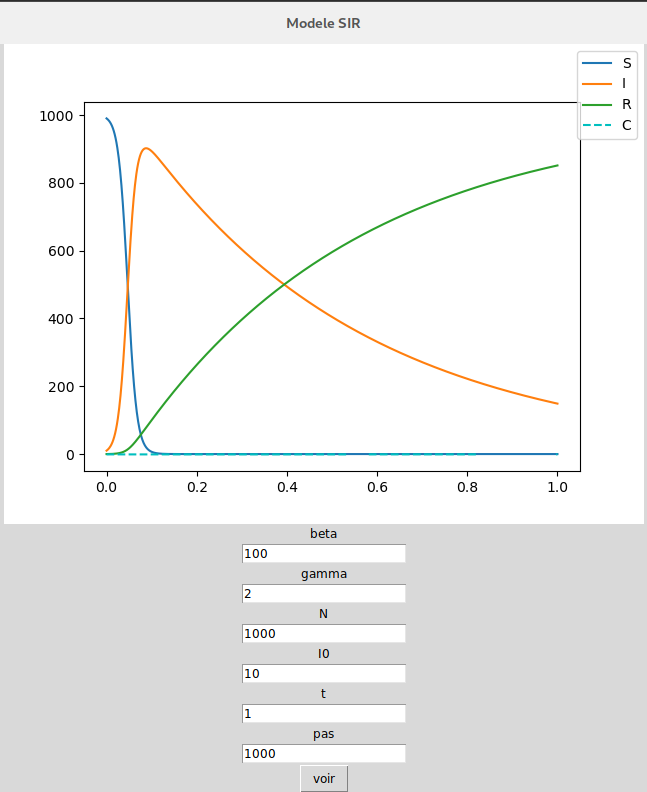
\includegraphics{forte_ep.png}
        \caption{Une forte épidémie}
    \end{minipage}
    \hfill%
    \begin{minipage}[c]{.46\linewidth}
        \centering
        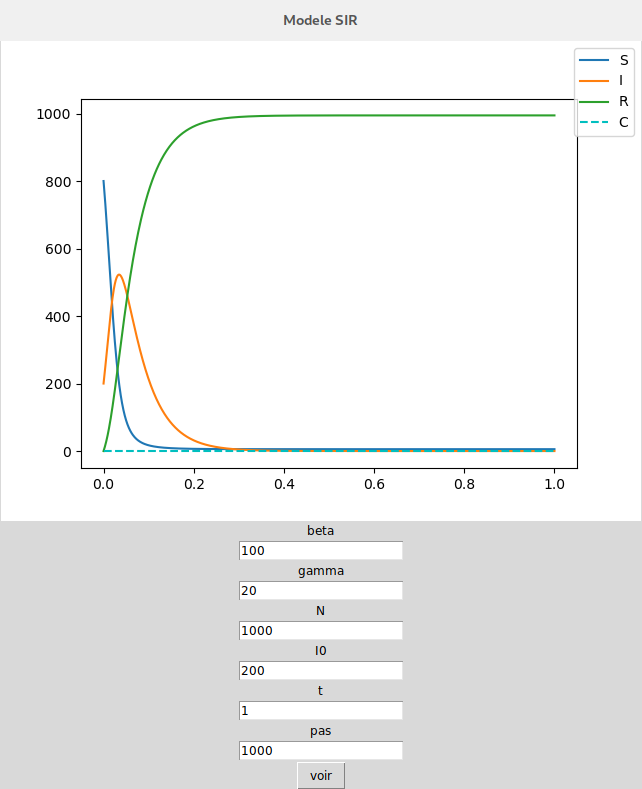
\includegraphics{faible_ep.png}
        \caption{Une épidémie plus faible}
    \end{minipage}
\end{figure}

\begin{figure}[h]
    \centering
    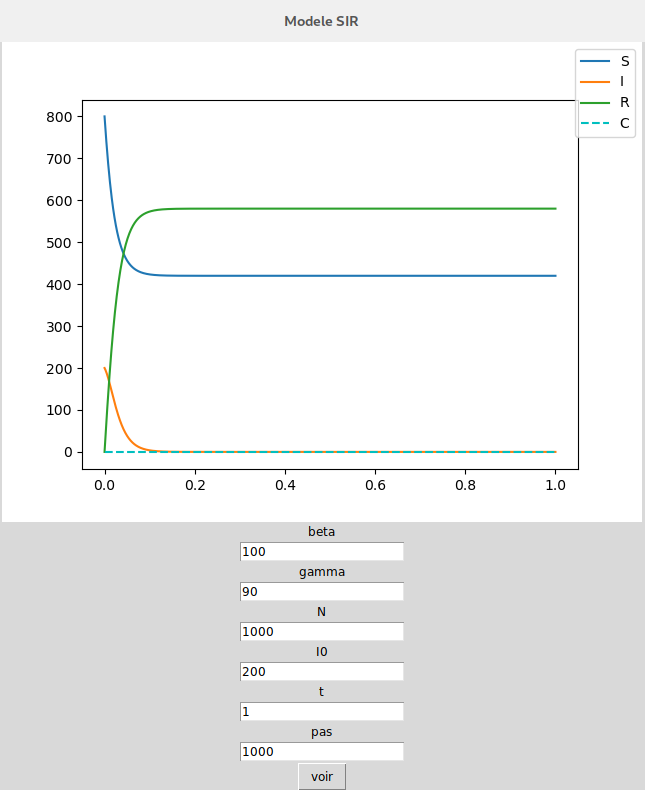
\includegraphics{fin_petite_ep.png}
    \caption{Une maladie qui se résorbe d'elle même}
\end{figure}{}


On peut également utiliser ce taux de reproduction pour comparer différentes maladies.

\begin{figure}[!h]
\begin{center}
   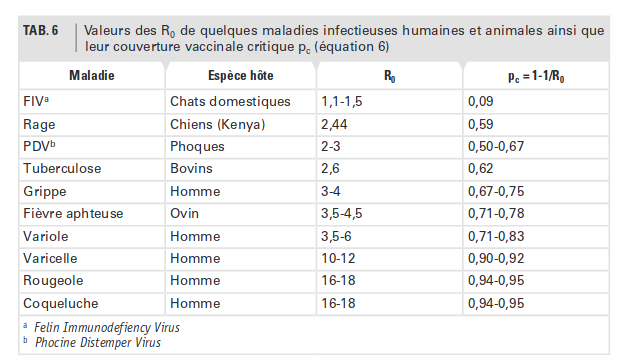
\includegraphics[scale= 0.6]{tab.png}
   \end{center}
\end{figure}





\section{Diffusion dans un graphe}
\subsection{Modélisation d'un réseau de transport: d'un modèle discret à un modèle continu}
%Utilisation de python, montrer qu'on est des pgms de la programmation : modelisation dehttp://marcchoisy.free.fr/pdf/DeBoeck2010.pdf graphs + animation de la transmission de l'epidemie si possible.
\subsubsection{Un réseau de transport}
Considérons un réseau de nœuds (par exemple des villes) et d’arêtes orientées (par exemple des lignes de train). On peut représenter ce réseau de transport par un graphe orienté et pondéré. En effet, pour un individu d'une ville $i$, il y a une probabilité $p_i^j$ d'aller vers la ville $j$, donc d'emprunter l’arête $i\rightarrow j$. 
%%graphe simpe avec des villes exemples

\tikzset{every picture/.style={line width=0.75pt}} %set default line width to 0.75pt        

\begin{tikzpicture}[x=0.75pt,y=0.75pt,yscale=-1,xscale=1]
%uncomment if require: \path (0,538); %set diagram left start at 0, and has height of 538

%Flowchart: Connector [id:dp9383929795512715] 
\draw   (31,128) .. controls (31,108.67) and (46.67,93) .. (66,93) .. controls (85.33,93) and (101,108.67) .. (101,128) .. controls (101,147.33) and (85.33,163) .. (66,163) .. controls (46.67,163) and (31,147.33) .. (31,128) -- cycle ;
%Flowchart: Connector [id:dp1847279895593108] 
\draw   (250,177) .. controls (250,157.67) and (265.67,142) .. (285,142) .. controls (304.33,142) and (320,157.67) .. (320,177) .. controls (320,196.33) and (304.33,212) .. (285,212) .. controls (265.67,212) and (250,196.33) .. (250,177) -- cycle ;
%Flowchart: Connector [id:dp002795637395967776] 
\draw   (324,97) .. controls (324,77.67) and (339.67,62) .. (359,62) .. controls (378.33,62) and (394,77.67) .. (394,97) .. controls (394,116.33) and (378.33,132) .. (359,132) .. controls (339.67,132) and (324,116.33) .. (324,97) -- cycle ;
%Flowchart: Connector [id:dp861794046635879] 
\draw   (337,300) .. controls (337,280.67) and (352.67,265) .. (372,265) .. controls (391.33,265) and (407,280.67) .. (407,300) .. controls (407,319.33) and (391.33,335) .. (372,335) .. controls (352.67,335) and (337,319.33) .. (337,300) -- cycle ;
%Flowchart: Connector [id:dp09586673435814774] 
\draw   (127,354) .. controls (127,334.67) and (142.67,319) .. (162,319) .. controls (181.33,319) and (197,334.67) .. (197,354) .. controls (197,373.33) and (181.33,389) .. (162,389) .. controls (142.67,389) and (127,373.33) .. (127,354) -- cycle ;
%Straight Lines [id:da5311713046534814] 
\draw    (101,128) -- (256.03,154.66) ;
\draw [shift={(258,155)}, rotate = 189.76] [color={rgb, 255:red, 0; green, 0; blue, 0 }  ][line width=0.75]    (10.93,-3.29) .. controls (6.95,-1.4) and (3.31,-0.3) .. (0,0) .. controls (3.31,0.3) and (6.95,1.4) .. (10.93,3.29)   ;

%Straight Lines [id:da12421349298198026] 
\draw    (66,163) -- (150.05,319.24) ;
\draw [shift={(151,321)}, rotate = 241.72] [color={rgb, 255:red, 0; green, 0; blue, 0 }  ][line width=0.75]    (10.93,-3.29) .. controls (6.95,-1.4) and (3.31,-0.3) .. (0,0) .. controls (3.31,0.3) and (6.95,1.4) .. (10.93,3.29)   ;

%Straight Lines [id:da14018417140139183] 
\draw    (261,204) -- (180.14,320.36) ;
\draw [shift={(179,322)}, rotate = 304.8] [color={rgb, 255:red, 0; green, 0; blue, 0 }  ][line width=0.75]    (10.93,-3.29) .. controls (6.95,-1.4) and (3.31,-0.3) .. (0,0) .. controls (3.31,0.3) and (6.95,1.4) .. (10.93,3.29)   ;

%Straight Lines [id:da6704769182504708] 
\draw    (311,153) -- (333.78,123.58) ;
\draw [shift={(335,122)}, rotate = 487.75] [color={rgb, 255:red, 0; green, 0; blue, 0 }  ][line width=0.75]    (10.93,-3.29) .. controls (6.95,-1.4) and (3.31,-0.3) .. (0,0) .. controls (3.31,0.3) and (6.95,1.4) .. (10.93,3.29)   ;

%Straight Lines [id:da25754741380563684] 
\draw    (296,214) -- (351.55,266.62) ;
\draw [shift={(353,268)}, rotate = 223.45] [color={rgb, 255:red, 0; green, 0; blue, 0 }  ][line width=0.75]    (10.93,-3.29) .. controls (6.95,-1.4) and (3.31,-0.3) .. (0,0) .. controls (3.31,0.3) and (6.95,1.4) .. (10.93,3.29)   ;

%Straight Lines [id:da5843093672750751] 
\draw    (324,97) -- (91,102.95) ;
\draw [shift={(89,103)}, rotate = 358.53999999999996] [color={rgb, 255:red, 0; green, 0; blue, 0 }  ][line width=0.75]    (10.93,-3.29) .. controls (6.95,-1.4) and (3.31,-0.3) .. (0,0) .. controls (3.31,0.3) and (6.95,1.4) .. (10.93,3.29)   ;

%Straight Lines [id:da7008965634161662] 
\draw    (359,132) -- (377.72,264.02) ;
\draw [shift={(378,266)}, rotate = 261.93] [color={rgb, 255:red, 0; green, 0; blue, 0 }  ][line width=0.75]    (10.93,-3.29) .. controls (6.95,-1.4) and (3.31,-0.3) .. (0,0) .. controls (3.31,0.3) and (6.95,1.4) .. (10.93,3.29)   ;

%Straight Lines [id:da25265663155293283] 
\draw    (191,334) -- (273.87,212.65) ;
\draw [shift={(275,211)}, rotate = 484.33] [color={rgb, 255:red, 0; green, 0; blue, 0 }  ][line width=0.75]    (10.93,-3.29) .. controls (6.95,-1.4) and (3.31,-0.3) .. (0,0) .. controls (3.31,0.3) and (6.95,1.4) .. (10.93,3.29)   ;

%Straight Lines [id:da9302149400895797] 
\draw    (254,166) -- (99.97,138.35) ;
\draw [shift={(98,138)}, rotate = 370.18] [color={rgb, 255:red, 0; green, 0; blue, 0 }  ][line width=0.75]    (10.93,-3.29) .. controls (6.95,-1.4) and (3.31,-0.3) .. (0,0) .. controls (3.31,0.3) and (6.95,1.4) .. (10.93,3.29)   ;

%Curve Lines [id:da3942851470598149] 
\draw    (50,96) .. controls (43.07,35.61) and (-19.73,95.77) .. (26.56,114.45) ;
\draw [shift={(28,115)}, rotate = 200.17000000000002] [color={rgb, 255:red, 0; green, 0; blue, 0 }  ][line width=0.75]    (10.93,-3.29) .. controls (6.95,-1.4) and (3.31,-0.3) .. (0,0) .. controls (3.31,0.3) and (6.95,1.4) .. (10.93,3.29)   ;

%Curve Lines [id:da5054855915884565] 
\draw    (394,86) .. controls (438.33,29.85) and (358.46,17.37) .. (366.57,59.06) ;
\draw [shift={(367,61)}, rotate = 255.95999999999998] [color={rgb, 255:red, 0; green, 0; blue, 0 }  ][line width=0.75]    (10.93,-3.29) .. controls (6.95,-1.4) and (3.31,-0.3) .. (0,0) .. controls (3.31,0.3) and (6.95,1.4) .. (10.93,3.29)   ;

%Curve Lines [id:da42066209622494355] 
\draw    (144,387) .. controls (127.17,427.59) and (215.21,423.1) .. (188.83,382.25) ;
\draw [shift={(188,381)}, rotate = 415.38] [color={rgb, 255:red, 0; green, 0; blue, 0 }  ][line width=0.75]    (10.93,-3.29) .. controls (6.95,-1.4) and (3.31,-0.3) .. (0,0) .. controls (3.31,0.3) and (6.95,1.4) .. (10.93,3.29)   ;

%Curve Lines [id:da7131082229155901] 
\draw    (350,329) .. controls (333.17,369.59) and (422.19,370.98) .. (395.83,330.25) ;
\draw [shift={(395,329)}, rotate = 415.38] [color={rgb, 255:red, 0; green, 0; blue, 0 }  ][line width=0.75]    (10.93,-3.29) .. controls (6.95,-1.4) and (3.31,-0.3) .. (0,0) .. controls (3.31,0.3) and (6.95,1.4) .. (10.93,3.29)   ;

%Straight Lines [id:da45370170325090897] 
\draw    (339,314) -- (198.93,353.46) ;
\draw [shift={(197,354)}, rotate = 344.27] [color={rgb, 255:red, 0; green, 0; blue, 0 }  ][line width=0.75]    (10.93,-3.29) .. controls (6.95,-1.4) and (3.31,-0.3) .. (0,0) .. controls (3.31,0.3) and (6.95,1.4) .. (10.93,3.29)   ;


% Text Node
\draw (64,130) node  [align=left] {Brest};
% Text Node
\draw (162,354) node  [align=left] {Toulouse};
% Text Node
\draw (285,177) node  [align=left] {Paris};
% Text Node
\draw (359,97) node  [align=left] {Lille};
% Text Node
\draw (372,300) node  [align=left] {Lyon};
% Text Node
\draw (64,145) node  [align=left] {1};
% Text Node
\draw (286,194) node  [align=left] {4};
% Text Node
\draw (360,116) node  [align=left] {2};
% Text Node
\draw (162,373) node  [align=left] {5};
% Text Node
\draw (372,317) node  [align=left] {3};
% Text Node
\draw (89,235) node  [align=left] {0,8};
% Text Node
\draw (175,132) node  [align=left] {0,1};
% Text Node
\draw (31,59) node  [align=left] {0,1};
% Text Node
\draw (203,85) node  [align=left] {0,4};
% Text Node
\draw (387,183) node  [align=left] {0,4};
% Text Node
\draw (412,34) node  [align=left] {0,2};
% Text Node
\draw (192,167) node  [align=left] {0,25};
% Text Node
\draw (304,131) node  [align=left] {0,25};
% Text Node
\draw (330,225) node  [align=left] {0,25};
% Text Node
\draw (222,234) node  [align=left] {0,25};
% Text Node
\draw (247,281) node  [align=left] {0,1};
% Text Node
\draw (177,433) node  [align=left] {0,9};
% Text Node
\draw (380,371) node  [align=left] {0,8};
% Text Node
\draw (280,318) node  [align=left] {0,2};

\label{graphe}
\end{tikzpicture}

Dans cette première partie, on ignore complètement le temps que passe un individu dans une ville. On considère le fait d'être dans une ville comme un état.\\

Sa matrice de transition est la matrice stochastique $V$:
$$
V=\begin{pmatrix}
0,1 &0& 0& 0,1 & 0,8\\
0,4 &0,2& 0,4& 0 & 0\\
0 &0& 0,8& 0 & 0,2\\
0,25 &0,25& 0,25& 0 & 0,25\\
0 &0& 0& 0,1 & 0,9
\end{pmatrix}
$$
Soit $E\subset\mathbb{N}$ l'ensemble des villes du réseau. Posons $(f_n)_{n=0}^{\infty}$ une suite de variables aléatoires sur $(\Omega, \tau, \mathbb{P})$ à valeurs dans $E$ qui indiquent dans quelle ville on se trouve au bout de $n$ transitions. Par construction, on suppose que la probabilité d'être dans une ville ne dépend que de la ville dans laquelle on était à l'étape précédente, et pas des autres. Ainsi, en notant $x_n$ la ville où l'on se trouve à l'étape $n$ et $f_n=x_n$ l'événement "se trouver dans la ville $x_n$ à l'étape $n$", on obtient
 $$\mathbb{P}(f_{n+1}=x_{n+1}|f_{n}=x_{n},f_{n-1}=x_{n-1},...,f_{0}=x_{0})=\mathbb{P}(f_{n+1}=x_{n+1}|f_{n}=x_{n})$$
La suite $(f_n)_{n=0}^{\infty}$ ainsi posée représente bien notre problème de transport. C'est une chaîne de Markov discrète homogène.
On ne considère ici que des graphes composés d'une seule composante connexe. En effet, étudier un graphe à $n$ composantes connexes revient à étudier $n$ graphes à une composante connexe.
\subsubsection{Introduction de la notion de temps}
Posons ${S(n), n\in\mathbb{N}}$ la séquence des temps de transition. C'est à dire que $S_n$ est l'instant auquel se produit la $n^{ieme}$ transition. On a bien évidement $S_0=0$ et $S_0<S_1<...<S_n<S_{n+1}<...$, mais il est difficile de déterminer la loi de $S$. En revanche on peut définir ${T(n), n\in\mathbb{N}}$ la séquence des temps de séjour. C'est à dire que $T_i(n)$ représente le temps qu'on reste dans une ville $i$ après la $n^{ieme}$ transition.\\
Ainsi, on a $T(n)=S(n+1)-S(n)$ mais aussi $S(n)=\sum_{m=0}^{n-1}T(m)$.\\
Précédemment, on a supposé que le fait de changer de ville, ici de passer d'un état à un autre, n'était pas conditionné par les villes déjà visitées. Il est donc cohérent de penser que $T_i$ suit une loi exponentielle, de facteur d'échelle $\nu_i$, qui dépend de la ville (on pourrait parler de coefficient d'attractivité, par exemple).\\
De plus, les transitions sont indépendantes les unes des autres, il en va donc de même pour les temps de séjours.
Avec ces hypothèses, on a que $\mathbb{P}(T_i(n)\leqslant t)$ est la probabilité de rester une période au plus $t$ dans la ville $i$.\\
Reprenons la chaîne de Markov $(f_n)_{n=0}^{\infty}$. Par simple changement d'indice, on peut poser $(\tilde{f_n})_{n=0}^{\infty}$, telle que $\tilde{f_n}=f_{S(n)}$. Alors $(\tilde{f_n})_{n=0}^{\infty}$ est une chaîne de Markov à temps discret homogène. Comme ${T(n), n\in\mathbb{N}}$ est une suite de variables aléatoires exponentielles indépendantes, on a construit ici une chaîne de Markov à temps continu.
\subsubsection{Étude de la chaîne de Markov à temps continu}
Considérons ${X(n), t\in\mathbb{R}^+}$ la chaîne de Markov à temps continu définie précédemment, et soit $E=\{0,r\}$ l'ensemble des états possibles (on se restreint ici à un ensemble fini d'états).\\
Posons $\vec{\pi}(t)$ le vecteur position au temps t. On a $\vec{\pi}(t)=\begin{bmatrix}
\pi_0(t)&...&\pi_r(t)
\end{bmatrix} $ tels que $$\pi_i(t)=\mathbb{P}(X(t)=i)$$ pour $i\in\{0,r\}$. \\
Et soit $P(t)$ la matrice de transition, telle que $$P(t)={\left( p_i^j (t) \right) }_{0\leq i\leq r}^{0\leq j\leq r}$$
Dans cette partie, on va expliciter le vecteur position et la matrice de transition en fonction du temps.
\paragraph{Équations de Kolmogorov}
Au sens strict, $ p_i^j (t)$ est la probabilité au temps $t$ de passer d'un état $i$ à un état $j$.\\
Soient $t_1$ et $t_2$ dans $\mathbb{R}^+$, tels que $t_1<t_2$
%%
\begin{align*}
p_i^j(t_1+t_2)&=\mathbb{P}(X(t_1+t_2)=j | X(0)=i)\\
&=\sum_{k\in E}\mathbb{P}(X(t_1+t_2)=j|X(t_1)=k,X(0)=i)\mathbb{P}(X(t_1)=k|X(0)=i)\\
&=\sum_{k\in E}\mathbb{P}(X(t_1+t_2)=j|X(t_1)=k)\mathbb{P}(X(t_1)=k|X(0)=i)\\
&=\sum_{k\in E}p_k^j(t_2)p_i^k(t_1)
\end{align*}
On reconnaît ici la formule du produit matriciel.\\
Considérons à présent $\pi_i(t)$, la probabilité d'être dans l'état $i$ au temps $t$. Alors pour les mêmes $t_1$ et $t_2$, on a
\begin{align*}
\pi_i(t_1+t_2)&=\mathbb{P}(X(t_1+t_2)=i)\\
&=\sum_{j\in E}p_k^i(t_1+t_2)\\
&=\sum_{j\in E}\sum_{k\in E}p_k^i(t_2)p_j^k(t_1)\\
&=\sum_{j\in E}\pi_j(t_1)p_k^i(t_2)
\end{align*}
\paragraph{Calcul explicite des probabilités de transition}
Si on revient à notre chaîne de Markov discrète $(f_n)_{n=0}^{\infty}$. Associons lui $Q$, une matrice de transition de coefficients $q_i^j$.\\
Soit $\Delta t$ un temps assez petit.\\
Supposons d'abord qu'il y ai effectivement transition durant le temps $\Delta t$. Autrement dit, prenons $i$ et $j$ dans $E$ tels que $i\neq j$.
Alors 

\begin{align*}
p_i^j(\Delta t)&=\mathbb{P}(X(\Delta t)=j|X(0)=i) \\
&=\mathbb{P}(T_i(0)\leqslant\Delta t)q_i^j\mathbb{P}(T_j(1)>\Delta t)
\end{align*}

%cette phrase est un peu bizzare%
C'est à dire que $p_i^j(\Delta t)$ est la probabilité de rester en $i$ au plus $\Delta t$, la probabilité que la transition de $i$ à $j$ ait lieu ($q_i^j$) et la probabilité de rester en $j$.\\
Or on sait que les $T$ suivent des lois exponentielles, donc:
$$
\mathbb{P}(T_i(0)\leqslant\Delta t)=(1-e^{-\nu_i\Delta t})
$$
et
$$\mathbb{P}(T_j(1)>\Delta t)=1-\mathbb{P}(T_j(1)\leqslant\Delta t)=1-(1-e^{-\nu_j\Delta t})=e^{-\nu_j\Delta t}$$
Or on ne s’intéresse qu'au comportement pour $\Delta t$ très petit. On peut donc approximer par un développement limité autour de 0.\\ On trouve:
$$\mathbb{P}(T_i(0)\leqslant\Delta t)\approx1-(1-\nu_i\Delta t+o(\Delta t))=\nu_i\Delta t+o(\Delta t)$$
et 
$$\mathbb{P}(T_j(1)>\Delta t)\approx1-\nu_j\Delta t+o(\Delta t)$$
Ainsi
\begin{align*}
p_i^j(\Delta t)&=(\nu_i\Delta t+o(\Delta t))q_i^j(1-\nu_j\Delta t+o(\Delta t))\\
&=q_i^j\nu_i\Delta t+o(\Delta t)
\end{align*}
Supposons à présent qu'il n'y ai pas eu de transition pendant cette période $\Delta t$. On va calculer $p_i^i(\Delta t)$ pour $i\in E$.
C'est donc la probabilité de rester plus que $\Delta t$ à l'état $i$ avant la première transition.\\
On a:
\begin{align*}
p_i^i(\Delta t)&=\mathbb{P}(X(\Delta t)=i|X(0)=i)\\
&=\mathbb{P}(T_i(0)>\Delta t)\\
&=1-1+e^{-\nu_i\Delta t}\\
&=e^{-\nu_i\Delta t}\\
&\approx 1-\nu_i\Delta t+o(\Delta t)
\end{align*}

On a ainsi trouvé une expression explicite pour chaque $p_i^j(\Delta t)$.
\paragraph{Explicitation de la dérivée du vecteur position}
Pour comprendre et analyser le modèle de diffusion en temps continue, on aimerait exprimer l'évolution de la population en chaque nœud du graphe, en chaque état, en fonction du temps. On cherche donc une expression de la dérivée du vecteur position $\vec{\pi}$.\\
On peut légitimement supposer que, pour un $\Delta t$ suffisamment petit, il n'y a qu'un seul changement d'état, qu'une seule transition.

Posons $t_2=\Delta t$, un temps très court, dans les équations de Kolmogorov obtenues précédemment.
Alors 
\begin{align*}
\pi_i(t+\Delta t)&=\sum_{k\in E}\pi_k(t)p_k^i(\Delta t)\\
&=\sum_{k\in E,k\neq i}\pi_k(t)p_k^i(\Delta t)+\pi_i(t)p_i^i(\Delta t)\\
&=\sum_{k\in E,k\neq i}\pi_k(t)(\nu_iq_k^i\Delta t+o(\Delta t))+\pi_i(t)(1-\nu_i\Delta t+o(\Delta t))\\
&=\sum_{k\in E,k\neq i}\pi_k(t)\nu_iq_k^i\Delta t +\pi_i(t)-\pi_i(t)\nu_i\Delta t + o(\Delta t)
\end{align*}
Donc
$$
\frac{\pi_i(t+\Delta t)-\pi_i(t)}{\Delta t}=\sum_{k\in E,k\neq i}\pi_k(t)q_k^i-\pi_i(t)\nu_i+\frac{o(\Delta t)}{\Delta t}
$$
En passant à la limite, on trouve exactement la définition de la dérivée de $\pi_i$, d'où:
$$
\frac{\mathrm{d}\pi_i}{\mathrm{d}t}(t)=\sum_{k\in E,k\neq i}\pi_k(t)q_k^i-\pi_i(t)\nu_i
$$
On reconnaît la forme d'un produit matriciel, avec les coefficients diagonaux négatifs. Ainsi, on peut poser 
$$M=
\begin{pmatrix}
-\nu_1^1 & \nu_1q_1^2&\hdots&\nu_1q_1^r\\
\nu_2q_2^1& -\nu_2^2&\hdots&\nu_2q_2^r\\
&&\ddots\\
\nu_rq_r^1&\nu_rq_r^2&\hdots&-\nu_r^r\\
\end{pmatrix}
$$
une matrice de transition, et exprimer:
$$\vec{\pi}'(t)=\vec{\pi}(t)M$$
Pour simplifier l'analyse du système dynamique ainsi obtenu, on étudiera $M^T$, qui a les mêmes valeurs propres que $M$, et on considérera le système suivant, avec les vecteurs colonnes:
$$\vec{\pi}'^T(t)=M^T\vec{\pi}^T(t)$$
\subsubsection{Quelques mots sur la matrice M}
\paragraph{liens entre les coefficients de M}
\paragraph{}$M$ n'est pas une matrice stochastique. En revanche, elle est construite à partir de la matrice stochastique $Q$. On peut en déduire une propriété sur les coefficients de $M$.
$p_i^j(t)$ est la probabilité de passer d'un état $i$ à un état $j$ au temps $t$. Ainsi, par la formule des probabilités totales, $\sum_{k\in E}p_i^k(\Delta t)=1$.
On rappelle que
\begin{align*}
    p_i^j(\Delta t)&=\nu_iq_i^j\Delta t+o(\Delta t) \text{      Pour }i\neq j\\
    p_i^i(\Delta t)&=1-\nu_i\Delta t+o(\Delta t)
\end{align*}
D'où:
\begin{align*}
   &\sum_{k\in E}p_i^k(\Delta t)=1\\
   \Longleftrightarrow &\sum_{k\in E,k\neq i}p_i^k(\Delta t)+1-\nu_i\Delta t=1+o(\Delta t)\\
   \Longleftrightarrow &\sum_{k\in E,k\neq i}\nu_iq_i^k\Delta t+1-\nu_i\Delta\\
   \Longleftrightarrow &\sum_{k\in E,k\neq i}\nu_iq_i^k-\nu_i=0\\
   \Longleftrightarrow &-\nu_i=-\sum_{k\in E,k\neq i}\nu_iq_i^k
\end{align*}

\paragraph{Somme des coefficients sur une ligne}
Par l'égalité précédente, on peut calculer la somme des coefficients de $M$ sur chaque ligne. Ainsi, $\sum_{k\in E}q_i^k=1$ pour chaque ligne $i$. Ainsi, pour une ligne $i$ de $M$ (dont on note $m_i^j$ le coefficient de la ligne $i$ et de la collone $j$):
$$
    \sum_{k\in E}m_i^k=\sum_{k\in E, k\neq i}\nu_iq_i^k-\nu_i=0$$
\paragraph{Constance de la population}
On aimerai s'assurer que la population sur notre graphe soit constante (voir, en fait, sur notre composante connexe). On s'assure donc que la somme des coefficients du vecteur de répartition de la population $\vec{\pi}$ soit une constante (donc que la dérivée de cette somme soit nulle). Ainsi on souhaite s'assurer que en tout $t\in \mathbb{R}^+$:
$$\sum_{k\in E}\pi_k(t)=N$$
\begin{align*}
\sum_{k\in E}\pi'_k(t)&=\sum_{k\in E}(\sum_{l\in E, l\neq k}\pi_l(t)\nu_kq_l^k-\pi_k(t)\nu_k)\\
&=\sum_{k\in E}\pi_k(t)(\sum_{l\in E, l\neq k}\nu_kq_k^l-\nu_k)\\
&=\sum_{k\in E}\pi_k(t)\times 0\\
&=0
\end{align*}
Ainsi, la population reste constante sur le graphe.\\
 \paragraph{Valeurs propres notables et multiplicité}
 On va étudier $M^T$, la transposée de $M$. ces deux matrices ont donc les mêmes valeurs propres.Comme les sommes sur chaque ligne des coefficients de $M$ sont nulles, il en va de même pour les sommes sur les collones de $M^T$. Ainsi toutes les lignes de $M^T$ sont linéairement dépendantes. $M^T$ n'est donc pas inversible, donc $0$ est une valeur propre de $M$.\\
 Trouvons maintaenant sa multiplicité. On rappelle que 
 $$m_{0}=dim(Ker(M))$$
 Et par la formule précédente, on a aussi
 \begin{align*}
   &-\nu_i=-\sum_{k\in E,k\neq i}\nu_iq_i^k\\
   \Longleftrightarrow &-\nu_i=-\nu_i\sum_{k\in E,k\neq i}q_i^k\\
    \Longleftrightarrow &-\nu_i=-\nu_i(1-q_i^i)
\end{align*}
Ainsi on peut réécrire $M$ comme:
$$M=
\begin{pmatrix}
-\nu_1(1-q_1^1) & \nu_1q_1^2&\hdots&\nu_1q_1^r\\
\nu_2q_2^1& -\nu_2(1-q_2^2)&\hdots&\nu_2q_2^r\\
&&\ddots\\
\nu_rq_r^1&\nu_rq_r^2&\hdots&-\nu_r(1-q_r^r)\\
\end{pmatrix}
$$
En simplifiant chaque ligne $i$ par $\nu_i$, on trouve $\Tilde{M}$, équivalente à $M$ (donc ayant les mêmes valeurs propres).
$$\Tilde{M}=
\begin{pmatrix}
(q_1^1-1) &q_1^2&\hdots&q_1^r\\
q_2^1& (q_2^2-1)&\hdots&q_2^r\\
&&\ddots\\
q_r^1&q_r^2&\hdots&(q_r^r-1)\\
\end{pmatrix}
$$
On cherche maintenant $dim(Ker(\Tilde{M}))$.\\
Or $\Tilde{M}=Q-I_k$ \\
Ainsi:
$$dim(Ker(M))=dim(Ker(\Tilde{M}))=dim(Ker(Q-I_k))$$
C'est la multiplicité de la valeur popre $1$ de la matrice stochastique $Q$! \\
$Q$ a une valeur propre qui vaut $1$ et sa multiplicité correspond au nombres de composantes connexes (de classes d'états closes) du graphe. Comme $M$ et $Q$ sont des matrices de transitions sur le même graphe (en temps continu et discret, respectivement), on a montré que la multiplicité de de la valeur propre $0$ de la matrice $M$ correspondait au nombre de composantes connexes du graphe.\\
Or on a supposé en introduction ne considérer que des graphes à une seule composante connexe. La multiplicité de la valeur propre $0$ est donc $1$.\\
De la même manière, 
\begin{align*}
    M-\lambda I_r&\sim\Tilde{M}-\lambda I_r\\
    &\sim Q-I_r-\lambda I_k\\
    &\sim Q-(\lambda +1)I_r
\end{align*}
Finalement, $\lambda$ est valeur propre de $M$ si et seulement si $\lambda +1$ est valeur propre de $Q$. Comme $Q$ est une matricte stochastique, on sait que $|\lambda +1|\leqslant1$.\\
Posons $\lambda=a+ib$. On aimerai déduire de la relation précédente une condition sur le signe de $a$, la partie réelle de $\lambda$.
On a alors:
\begin{align*}
   &|\lambda +1|\leqslant1\\
  \Leftrightarrow&|a+1+ib|\leqslant1\\
  \Leftrightarrow&\sqrt{(a+1)^2+b^2}\leqslant1\\
  \Leftrightarrow&(a+1)^2+b^2\leqslant1\\
\end{align*}
Posons $a\geq0$.\\
Alors
\begin{align*}
    \Leftrightarrow&a^2+2a+1+b^2\leqslant1\\
    \Leftrightarrow&a^2+2a+b^2\leqslant0\\
\end{align*}
C'est une contradiction car $2a\geq0$. On a alors prouvé que toutes les valeurs propres de $M$ ont une partie réelle négative ou nulle.
\subsection{Convergence du modèle}
\subsubsection{Existence et unicité de la solution}
\begin{thm}
Soient $t_0\in \mathbb{R}$ et $x_0\in \mathbb{R}^n$ et $A\in \mathbb{R}^n\times\mathbb{R}^n$. L'unique solution de l'équation $x'(t)=Ax(t)$ valant $x_0$ en $t_0$ est l'application $x$ définie par
$$x(t)=e^{(t-t_0)A}x_0,      \forall t\in \mathbb{R}$$
\end{thm}
L'équation ) correspond bien aux conditions d'application du théorème. Ainsi il existe une unique application $\vec{\pi}^T$ qui décrit le déplacement de la population sur un graphe pour une répartition à un temps initial $t_0$: $\vec{\pi}^T(t_0)$. \\
Il est évident que l'allure de la solution dépendra de l'exponentielle de la matrice $M^T$. \\
Pour rappel, pour $A$ une matrice carrée de taille $n\times n$, $e^A=\sum_{k=0}^{\infty}\frac{A^k}{k!}$.\\
Soit $\vec{\pi}(t)=e^{tM^T}\vec{\pi}(0)$, la solution du problème de Cauchy(**) pour $t\in\mathbb{R}^+$.\\
\subsubsection{Etude de la solution}
\paragraph{Formule explicite de la solution}
On a déjà montré que $0$ était une valeur propre de $M$, de multiplicité le nombre de composantes connexes du graphe. Ainsi $M^T$ n'est pas diagonalisable. En revanche, on peut toujours en déterminer une décomposition de Jordan.\\
Soit $J_\lambda$ le bloc de Jordan associé à la valeur propre $\lambda$ de multiplicité $m_\lambda$. Alors $J_\lambda$ est une matrice carrée $m\times m$ de la forme:
$$J_\lambda=\begin{pmatrix}
 \lambda& 1 &0& ... & 0\\
 0 & \lambda&1& ...&0\\
 \vdots&&\ddots&\ddots&\vdots\\
 0&...&0&\lambda&1\\
 0&...&&0&\lambda\\
\end{pmatrix}$$
On peut alors écrire $J_\lambda=\lambda I_m+N_m$, où $N_m$ est la matrice $m\times m$ telle que 
$$N_m=\begin{pmatrix}
 0& 1 &0& ... & 0\\
 0 & 0&1& ...&0\\
 \vdots&&\ddots&\ddots&\vdots\\
 0&...&0&0&1\\
 0&...&&0&0\\
\end{pmatrix}$$
Ainsi il existe $D$ une matrice nulle sauf sur sa diagonale qui est composée des blocs de Jordan associés à chacunes des valeurs propres de $M^T$ et $P$ une matrice inversible telles que $M^T=PDP^{-1}$.
\paragraph{Exponentielle de $M^Tt$}
pour déterminer explicitement la solution du problème de Cauchy (**), il faut calculer $$e^{tM^T}=\sum_{k=0}^{\infty}\frac{t^k (M^T)^k}{k!}$$
Or avec la décomposition de Jordan de $M^T$ on a:
\begin{align*}
    e^{tM^T}&=\sum_{k=0}^{\infty}\frac{t^k(M^T)^k}{k!}\\
    &=\sum_{k=0}^{\infty}\frac{t^k(PDP^{-1})^k}{k!}\\
    &=P\left(\sum_{k=0}^{\infty}\frac{t^kD^k}{k!}\right)P^{-1}\\
    &=Pe^{tD}P^{-1}\\
\end{align*}
Ainsi, pour calculer l'exponentielle de $tM^T$ il suffitde calculer l'exponentielle de la matrice $D$ de la décomposition de Jordan.\\
$D$ est diagonale par blocs, ainsi 
$$
D^k=\begin{pmatrix}
J_{\lambda_1}^k&0&\hdots&0\\
0&J_{\lambda_2}^k&\hdots&0\\
\vdots&\ddots&\ddots&\vdots\\
0&\hdots&0&J_{\lambda_i}^k\\
\end{pmatrix}
$$
Ainsi $e^{tD}=\begin{pmatrix}
e^{tJ_{\lambda_1}}&0&\hdots&0\\
0&e^{tJ_{\lambda_2}}&\hdots&0\\
\vdots&\ddots&\ddots&\vdots\\
0&\hdots&0&e^{tJ_{\lambda_i}}\\
\end{pmatrix}$ 
Le problème revient donc à calculer l'exponentielle d'un bloc de Jordan.\\
Soit $J_\lambda$ un bloc de Jordan de taille $m$. On a alors:
$$J_\lambda=\lambda I_m+N_m$$
Comme $I_m$ commute avec toutes les matrices de taille $m \times m$, et en particulier $N_m$, on a:
\begin{align*}
    e^{tJ_\lambda}&=e^{t\left(\lambda I_m+N_m\right)}\\
    &=e^{t\lambda I_m}\times e^{tN_m}\\
    &=e^{t\lambda}I_m\times e^{tN_m}
\end{align*}
Determinons une formule générale pour $e^{tN_m}$:\\
One note que $N_m^k$ est nulle si $k\geqslant m$ et vaut la matrice dont la $k$ième diagonale est 1 et le reste 0 sinon.
(**preuve en annexe**)\\
Ainsi:
$$
    e^{tN_m}=\begin{pmatrix}
1 & t& \frac{t^2}{2} & \cdots & \frac{t^{p-1}}{(p-1)!} \\
0 & \ddots&\ddots & \ddots & \vdots \\
\vdots & \ddots & \ddots &t& \frac{t^2}{2} \\
\vdots & 0&\ddots & \ddots & t \\
0 & \cdots&\cdots & 0 & 1 \\ \end{pmatrix}$$
D'où 
\begin{align*}
    e^{tJ_\lambda}&=e^{t\lambda}I_m\times e^{tN_m}\\
    &=e^{t\lambda}\times \begin{pmatrix}
1 & t& \frac{t^2}{2} & \cdots & \frac{t^{p-1}}{(p-1)!} \\
0 & \ddots&\ddots & \ddots & \vdots \\
\vdots & \ddots & \ddots &t& \frac{t^2}{2} \\
\vdots & 0&\ddots & \ddots & t \\
0 & \cdots&\cdots & 0 & 1 \\ \end{pmatrix}
\end{align*}

\begin{comment}
\paragraph{Matrices diagonalisables}
Soit $A\in Mn(\mathbb{R})$ une matrice diagonalisable. Alors il existe $P\in GLn(\mathbb{R})$ et $D\in Mn(\mathbb{R})$ diagonale telles que $A=PDP^{-1}$.\\
La matrice $D$ ainsi déterminée est la matrice diagonale de la forme 
$$D=\begin{pmatrix}
 \lambda_1 & 0 & ... & 0\\
 0 & \lambda_2 & ...&0\\
 \vdots&&\ddots&\vdots\\
 0&...&0&\lambda_n\\
\end{pmatrix}$$
Où les $\lambda_i$ sont les valeurs propres de la matrice $A$.\\
On en profite pour expliciter 
$$D^k=\begin{pmatrix}
 \lambda_1^k& 0 & ... & 0\\
 0 & \lambda_2^k& ...&0\\
 \vdots&&\ddots&\vdots\\
 0&...&0&\lambda_n^k\\
\end{pmatrix}$$
On a alors que $e^A=e^{PDP^{-1}}$\\
Or par récurrence, on montre aisément que $A^k=PD^kP^{-1}, \forall k\in \mathbb{N}$.\\
Ainsi
\begin{align*}
e^{(t-t_0)A}&=e^{(t-t_0)PDP^{-1}}\\
&=\sum_{k=0}^{\infty}\frac{((t-t_0)A)^k}{k!}\\
&=\sum_{k=0}^{\infty}\frac{((t-t_0)PDP^{-1})^k}{k!}\\
&=\sum_{k=0}^{\infty}\frac{P((t-t_0)D)^kP^{-1}}{k!}\\
&=P\sum_{k=0}^{\infty}\frac{((t-t_0)D)^k}{k!}P^{-1}\\
&=P\sum_{k=0}^{\infty}\frac{1}{k!}\begin{pmatrix}
 ((t-t_0)\lambda_1)^k& 0 & ... & 0\\
 0 & ((t-t_0)\lambda_2)^k& ...&0\\
 \vdots&&\ddots&\vdots\\
 0&...&0&((t-t_0)\lambda_n)^k\\
\end{pmatrix}P^{-1}\\
\end{align*}
On trouve alors $$e^{(t-t_0)A}=P\begin{pmatrix}
 e^{(t-t_0)\lambda_1}& 0 & ... & 0\\
 0 & e^{(t-t_0)\lambda_2}& ...&0\\
 \vdots&&\ddots&\vdots\\
 0&...&0&e^{(t-t_0)\lambda_n}\\
\end{pmatrix}P^{-1}$$

\paragraph{Matrices non-diagonalisables}
Dans le cas où la matrice $A$ ne serai pas diagonalisable, on peut utiliser la décomposition de Jordan. \\
-----------------exponentiel d'un bloc de Jordan--------------------\\
\end{comment}

\paragraph{Convergence de la solution}
La solution du problème de Cauchy (**) est $u(t)Pe^{tD}P^{-1}\pi(0)$ avec $P$ une matrice inversible et $D$ une matrice diagonale par bloc composée de bloc de Jordan.\\
De plus cette solution est définie pout $t\in \mathbb{R}^+$. 
\begin{align*}
    \lim\limits_{t \rightarrow +\infty}\vec{\pi}(t)&=\lim\limits_{t \rightarrow +\infty}Pe^{tD}P^{-1}\pi(0)\\
    \\
    &=P\left(\lim\limits_{t \rightarrow +\infty}e^{tD}\right)P^{-1}\pi(0)\\
    \\
    &=P\lim\limits_{t \rightarrow +\infty}\begin{pmatrix}
e^{tJ_{\lambda_1}}&0&\hdots&0\\
0&e^{tJ_{\lambda_2}}&\hdots&0\\
\vdots&\ddots&\ddots&\vdots\\
0&\hdots&0&e^{tJ_{\lambda_i}}\\
\end{pmatrix}P^{-1}\pi(0)\\
\\
&=P\begin{pmatrix}
\lim\limits_{t \rightarrow +\infty}e^{tJ_{\lambda_1}}&0&\hdots&0\\
0&\lim\limits_{t \rightarrow +\infty}e^{tJ_{\lambda_2}}&\hdots&0\\
\vdots&\ddots&\ddots&\vdots\\
0&\hdots&0&\lim\limits_{t \rightarrow +\infty}e^{tJ_{\lambda_i}}\\
\end{pmatrix}P^{-1}\pi(0)\\
\end{align*}
Or pour $J_\lambda$ un bloc de Jordan de taille $m\times m$:
\begin{align*}
    \lim\limits_{t \rightarrow +\infty}e^{tJ_{\lambda}}&=\lim\limits_{t \rightarrow +\infty}e^{t\lambda}\times \begin{pmatrix}
1 & t& \frac{t^2}{2} & \cdots & \frac{t^{p-1}}{(p-1)!} \\
0 & \ddots&\ddots & \ddots & \vdots \\
\vdots & \ddots & \ddots &t& \frac{t^2}{2} \\
\vdots & &\ddots & \ddots & t \\
0 & \cdots&\cdots & 0 & 1 \\ \end{pmatrix}
\end{align*}

\paragraph{bloc de Jordan associé à la valeur propre 0}
On a déjà expliqué que les multipliciés algébriques et géométriques de $0$ valaient $1$. Ainsi $J_0=\begin{pmatrix}
1
\end{pmatrix}$ pour tout $t\in\mathbb{R}^+$
\paragraph{Bloc de Jordan associé à une valeur propre réelle}
On a prouvé que toutes les parties réelles des valeurs propres non-nulles de $M$ étaient strictement négatives. De plus, par les croissances comparées, en comme $t$ est positif:
\begin{align*}
    \lim\limits_{t \rightarrow +\infty}e^{tJ_{\lambda}}&=\lim\limits_{t \rightarrow +\infty}e^{t\lambda}\times \begin{pmatrix}
1 & t& \frac{t^2}{2} & \cdots & \frac{t^{p-1}}{(p-1)!} \\
0 & \ddots&\ddots & \ddots & \vdots \\
\vdots & \ddots & \ddots &t& \frac{t^2}{2} \\
\vdots & &\ddots & \ddots & t \\
0 & \cdots&\cdots & 0 & 1 \\ \end{pmatrix}\\
\\
&= \lim\limits_{t \rightarrow +\infty}e^{t\lambda}\times \begin{pmatrix}
1 & 1& 1 & \cdots & 1\\
1 & \ddots&\ddots & \ddots & \vdots \\
\vdots & \ddots & \ddots &1& 1 \\
\vdots & &\ddots & \ddots & 1 \\
0 & \cdots&\cdots & 0 & 1 \\ \end{pmatrix}\\
\end{align*}
Or $$\lim\limits_{t \rightarrow +\infty}e^{t\lambda}=0$$
D'où
$$\lim\limits_{t \rightarrow +\infty}e^{tJ_{\lambda}}=0_{\mathcal{M}_{p,p}(\mathbb{R})}$$
\paragraph{Bloc de Jordan associé à une valeur popre complexe}
De la même maniére, si $\lambda =\alpha +i\beta$, avec $\alpha<0$, on a:
\begin{align*}
    e^{t\lambda}&=e^{t(\alpha +i\beta)}\\
    &=e^{t\alpha}\times e^{ti\beta}\\
    &=e^{t\alpha}\left(cos(t\beta)+isin(t\beta)\right)
\end{align*}
Toujours par croissances comparées, on a: 
$$\lim\limits_{t \rightarrow +\infty}e^{t\lambda}=\lim\limits_{t \rightarrow +\infty}e^{t\alpha}=0$$
Ainsi on trouve à nouveau
$$\lim\limits_{t \rightarrow +\infty}e^{tJ_{\lambda}}=0_{\mathcal{M}_{p,p}(\mathbb{R})}$$
\paragraph{Existence et interprétation de la limite}
On a prouvé que le seul bloc de Jordan dont la limite est non-nulle est celui de dimension 1 associé à la valeur propre nulle. \\
On a alors, en supposant qu'on ai placé le bloc de Jordan associé à 0 en première position:
\begin{align*}
\lim\limits_{t \rightarrow +\infty}\vec{\pi}(t)&=P\lim\limits_{t \rightarrow +\infty}\begin{pmatrix}
e^{tJ_{\lambda_1}}&0&\hdots&0\\
0&e^{tJ_{\lambda_2}}&\hdots&0\\
\vdots&\ddots&\ddots&\vdots\\
0&\hdots&0&e^{tJ_{\lambda_i}}\\
\end{pmatrix}P^{-1}\pi(0)\\
\\
&=P\lim\limits_{t \rightarrow +\infty}\begin{pmatrix}
e^{tJ_{0}}&0&\hdots&0\\
0&0&\hdots&0\\
\vdots&\ddots&\ddots&\vdots\\
0&\hdots&0&0\\
\end{pmatrix}P^{-1}\pi(0)\\
\\
&=P\begin{pmatrix}
1&0&\hdots&0\\
0&0&\hdots&0\\
\vdots&\ddots&\ddots&\vdots\\
0&\hdots&0&0\\
\end{pmatrix}P^{-1}\pi(0)\\
\end{align*}
Ainsi la limite en l'infinie dépend du vecteur propre associé à la valeur propre 0 et de la distribution initiale.
\newpage
\section{Epidémie sur un graphe et analyse numérique}
\subsection{Le modèle SIR sur notre modèle de diffusion}
On aimerait maintenant représenter la propagation d'une épidémie sur un graphe, au sein d'une population qui se déplace. Au lieu d'étudier le vecteur des positions $\pi$, on va étudier trois vecteurs de $\mathbb{R}^r$ avec $r$ le nombre de noeuds du graphe, représentant chacun les positions d'une catégorie de la population (Sain, Infecté ou Remis). On appelle ces vecteurs $\vec{S}$, $\vec{I}$ et $\vec{R}$. Ainsi, la composante $S_i(t)$ représente la population saine au noeud $i$ au temps $t$.
\paragraph{En supposant les villes non-reliées} On considère $r$ épidémies au sein de $r$ populations indépendantes. En utilisant les systèmes dynamiques présentés en première partie, on a, pour chaque ville $i$:
\begin{align}
    \frac{\mathrm{d}S_i}{\mathrm{d}t}(t)&=-\beta S_i(t)I_i(t)\\
    \frac{\mathrm{d}I_i}{\mathrm{d}t}(t)&=\beta S_i(t)I_i(t)-\gamma I_i(t)\\
    \frac{\mathrm{d}R_i}{\mathrm{d}t}(t)&=\gamma I_i(t)
\end{align}
Les vecteurs sont donc de la forme:
\begin{align}
    \vec{S'}(t)&=-\beta \vec{S}(t)\circ\vec{I}(t)\\
   \vec{I'}(t)&=\beta \vec{S}(t)\circ\vec{I}(t)-\gamma \vec{I}(t)\\
    \vec{R'}(t)&=\gamma \vec{I}(t)
\end{align}
Avec $\circ$, l'opérateur pour le produit composante par composante.
\paragraph{En supposant les villes reliées} On prend maintenant en compte les déplacement de la population entre les noeuds du graphe. Dans la partie 3, on a déterminé le système dynamique 
$$\vec{\pi'}(t)=\vec{\pi}(t)M$$
avec $M$ une matrice $r\times r$ et $\vec{\pi}$ le vecteur position.\\
Pour unir ces deux modèles, on va considérer trois catégories de populations (non indépendantes) qui se déplacent (éventuellement avec des vitesses différentes, qu'on peut noter $d_S$, $d_I$ et $d_R$. Par exemple un individu sain pourrait se déplacer dix fois plus rapidement qu'un individu infecté).\\
Ainsi, à $t+\Delta t$, les populations des trois catégories correpondent aux populations de ces catégories au temps $t$, plus les variations duent à:
\begin{itemize}
    \item La population nouvellement arrivée/partie\\
    \item Les transmissions et rémissions de la population, liées à l'évolution de l'épidémie\\
\end{itemize}
Le système ainsi défini devient donc:
\begin{align}
    \vec{S'}(t)&=d_S\vec{S}(t)M-\beta \vec{S}(t)\circ\vec{I}(t)\\
   \vec{I'}(t)&=d_I\vec{I}(t)M+\beta \vec{S}(t)\circ\vec{I}(t)-\gamma \vec{I}(t)\\
    \vec{R'}(t)&=d_R\vec{R}(t)M+\gamma \vec{I}(t)
\end{align}
L'introduction de ces coefficients de vitesse de déplacement permettent la modèlisation d'une épidèmie de maladies avec un impact physique important sur les individus, mortelles notamment en posant $d_R=0$.

Maintenant qu'on a analysé les modèles de diffusion, on souhaite s'en servir pour générer des modèles dynamiques.
\subsection{Méthodes numériques}
On cherche une méthode qui permette de résoudre une équation différentielle. On remarque d'ailleurs que toutes les équations différentielles étudiées ici sont homogènes, on peut donc les écrire comme:
$$\vec{y'}(t)=f(\vec{y}(t))$$
avec $f$ une application de $\mathbb{R}^n$ dans $\mathbb{R}^n$.\\
Pour alléger l'écriture, on écrit $y$ au lieu de $\vec{y}$, en considérant que la dimension de $y$ reste cohérente.
Or par définition de la limite: 

\begin{align*}
y'(t)&=\frac{y(t+h)-y(t)}{h}\\
\Longleftrightarrow f(y(t))&=\frac{y(t+h)-y(t)}{h}\\
\Longleftrightarrow hf(y(t))&=y(t+h)-y(t)\\
\Longleftrightarrow y(t+h)&=y(t)+hf(y(t))
\end{align*}
\subsubsection{Méthode d'Euler}
Par récursion en partant des valeurs initiales, on peut construire une solution à l'équation différentielles $y'(t)=f(y(t))$.\\
Soit $(t_n)_{n\in\mathbb{N}}$ une suite croissante de points en lesquels on veut estimer la solution du problème de Cauchy, avec $t\in \mathbb{R}^+$. On a la relation par récurence:
\begin{align}
    y(t_0)&=y_0\\
    y(t_{n+1})&=y(t_n))+(t_{n+1}-t_n)f(y(t_n))
\end{align}
On peut implémenter cette méthode de résolution en Python en générant une suite $(t_n)_{n\in\mathbb{N}}$ telle que 
\begin{align*}
  t_0&=t_0\\
  t_{n+1}&=t_n+h
\end{align*}
\begin{verbatim}
def euler(t0,Npas,h,y0,f):
    n= np.arange(t0,Npas,h)
    y=[]
    y[t0]=y0
    for i in range (len(n)):
        t=i*h
        y[i+1]=y[i]+h*f(t,y[i])
    return y
\end{verbatim}


\subsubsection{Méthode du point milieu}
Le but de cette méthode est d'être plus fine que la méthode d'Euler. Ainsi, au lieu d'approximer par la valeur de $f$ en $y_n$, on approxime par la valeur de $f$ entre $y_n$ et $y_{n+1}$. 

$$y_{n+1} = y_n + h f \left(y_n + \frac{h}{2} f \left( t, y_n \right) \right)$$

\begin{verbatim}
    def point_milieu(t0,Npas,h,y0,f):
    d=h/2
    n= np.arange(t0,Npas,h)
    y=[]
    y[t0]=y0
    for i in range (len(n)):
        t=i*h
        y[i+1]=y[i]+h*f(t+d,y[i]+df(t,y[i]))
    return y
\end{verbatim}

\subsubsection{Méthode de Runge-Kutta d'ordre 4}
La méthode de Runge-Kutta générale repose sur le principe de l'itération. On  va donc calculer une première estimation de la solution, puis l'utilisée pour calculer une seconde estimation, plus précise, et ainsi de suite. C'est une méthode à $q$ pas. Ainsi plus il y a d'itération, plus notre construction se rapprochera de la solution. Cela dit, plus il y a d'itérations, plus le calcul de la solution est fastidieux, et au delà d'un certain ordre, la précision gagnée n'est plus forcément intéressante par rapport aux nombres d'étapes nécéssaires. 

Nous nous intéressons à la méthode de Runge-Kutta d'orde 4. 
La méthode est la suivante : $$y_{n+1}= y_n+\frac{h}{6}(k_1+2k_2+2k_3+k_4)$$
où \begin{align*}
    k_1&=f(t_n,y_n)\\
    k_2&=f(t_n+\frac{h}{2},y_n+\frac{h}{2}k_1)\\
    k_3&=f(t_n+\frac{h}{2},y_n+\frac{h}{2}k_2)\\
    k4_&=f(t_n+h,y_n+h k_3)
\end{align*}

\begin{verbatim}
    def rk(t0,y0,pas,Npas,f):
    n=np.arange(t0,Npas,pas)
    y=[]
    y[0]=y0
    tmp2=0
    tmp3=0
    tmp4=0
    p=range(1,4)
    for i in range (len(n)):
        t=i*pas
        p[1]=f(t,y[i])
        tmp2=y[i]+(pas/2)*p[1]
        p[2]=f(t+pas/2,tmp2)
        tmp3=y[i]+(pas/2)*p[2]
        p[3]=f(t+pas/2,tmp3)
        tmp4=y[i]+pas*p[3]
        p[4]=f(t+h,tmp4)
        y[i+1]=y[i]+pas/6(p[1]+2*p[2]+2*p[3]+p[4])
    return y
\end{verbatim}

En fait, les méthodes d'Euler et du point milieu sont des cas particuliers de la méthode de Runge Kutta (d'orde 1 et 2). 
\newpage
\subsection{Représentations et comparaison des méthodes}

\begin{figure}[h!]
    \centering
    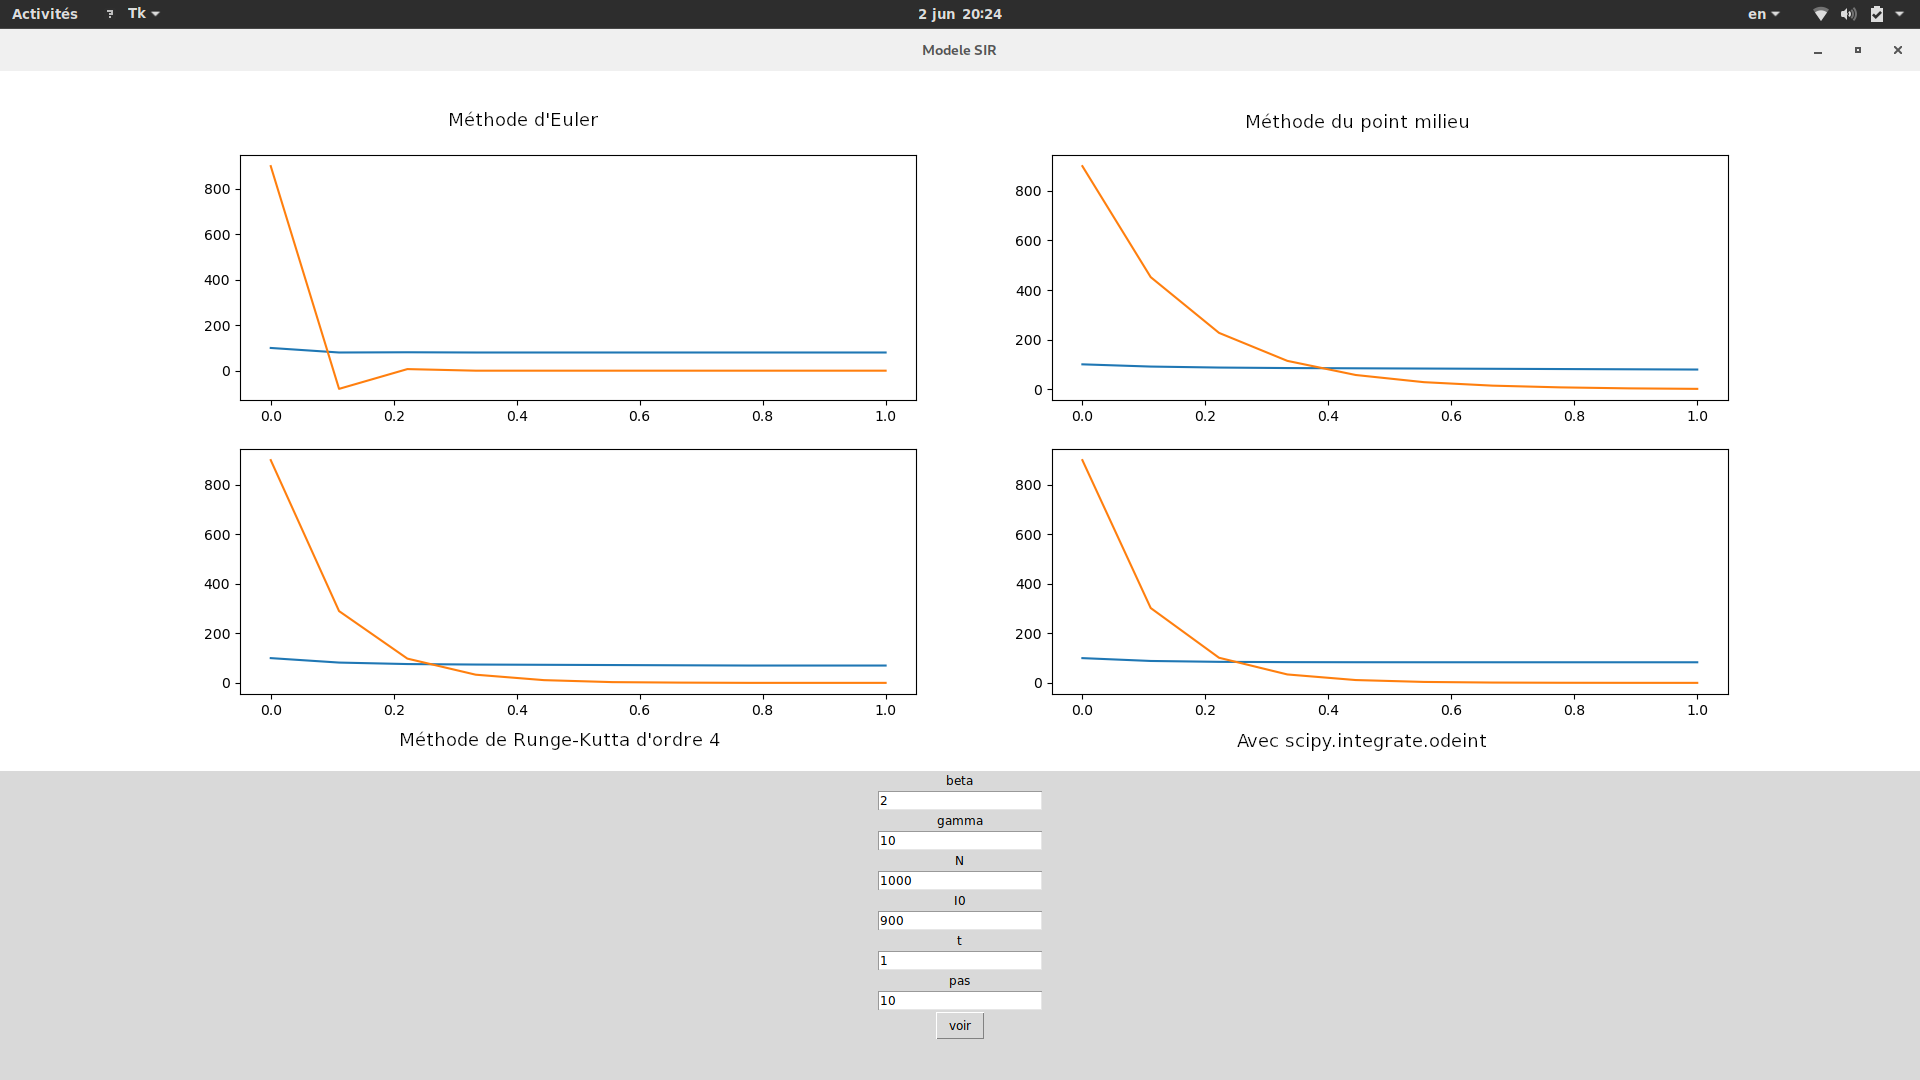
\includegraphics{comp2.png}
    \caption{Comparaison des méthodes avec un petit nombre de pas}
\end{figure}{}

On peut voir sur la figure ci dessus qu'avec un petit nombre de pas, la méthode d'Euler est peu fiable, c'est la plus éloignée de la solution.
\begin{figure}[h!]
    \centering
    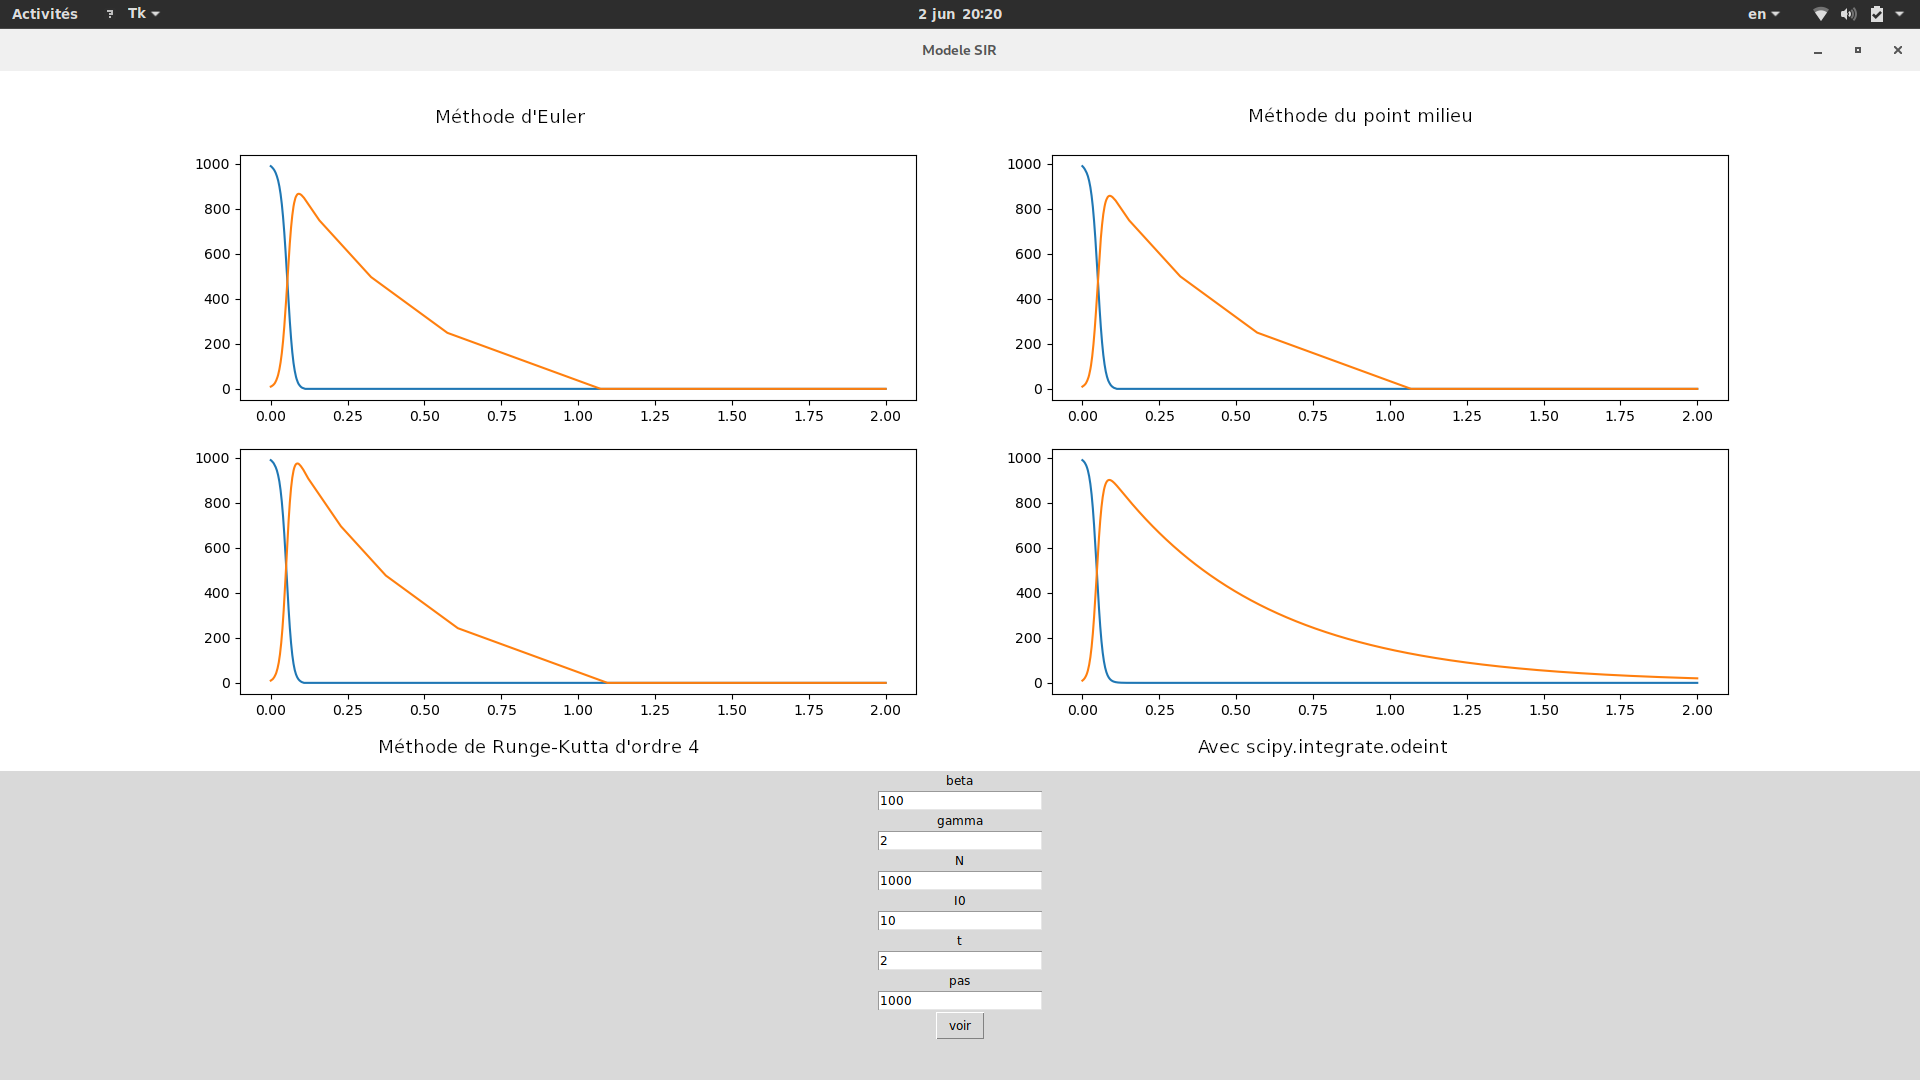
\includegraphics{comp1.png}
    \caption{Comparaison des méthodes avec un grand nombre de pas}
\end{figure}{}

Avec un grand nombre de pas en revanche, on peut noter que nos 3 méthodes se rapprochent sensiblement de la solution.


\section{Conclusion}
Dans un premier temps, nous avons construit et étudié un modèle de diffusion simple d'une épidémie dans une population fixe. Nous nous sommes rendu compte de l'existence qu'une épidémie avait lieu lorsque certaines conditions étaient respectées, et étudier son évolution. Nous avons pu notamment nous intéresser rapidement à la question de la vaccination, pour éviter les épidémies.

Nous avons ensuite étudié la répartition en fonction du temps d'une population sur un graphe, en construisant des chaînes de Markov continues.
La combinaison de ces deux modèles nous a permis d'analyser des situations plus complexes, et de simuler la propagation de la maladie dans une population en mouvement.

La question reste ouverte sur la quarantaine, sur un réseau de transport par exemple, quels axes faudrait-il supprimer pour endiguer l'évolution de la maladie? Ou encore s'intéresser à un modèle plus complexe comme par exemple le modèle SEIRS, dans lequel on prend en compte le temps d'exposition à la maladie et une fois guéri on peut recontracter la maladie. Il serait également intéressant de se pencher sur les modèles tenant compte de la démographie naturelle, pour comprendre un champs plus large de la propagation des maladies.

Nous avons grandement apprécié travailler sur ce sujet, et en apprendre d'avantage sur un phénomène qui nous concerne tous.

Nous tenons également à remercier Mr Alessandro Zilio, pour son encadrement et ses explications sur les nouveautés que nous avons pu aborder. 
\newpage
\section{Bibliographie/Sources}

\href{http://www.fields.utoronto.ca/video-archive/static/2018/03/2365-18260/mergedvideo.ogv}{Uncovering the epidemic pattern of medieval plagues}

\href{http://marcchoisy.free.fr/pdf/DeBoeck2010.pdf}{Modélisation mathématique en épidémiologie}

\href{https://link-springer-com.rproxy.sc.univ-paris-diderot.fr/content/pdf/10.1007%2F978-1-4757-3516-1.pdf?fbclid=IwAR21g7kvo-btJQpJCJuV5iVIisr7WpWtXjJ77LII1XvINunnGlIuqqYSDT8}{Mathematical Models in Population Biology and Epidemiology, Fred Brauer,Carlos Castillo-Chavez}

\href{https://docplayer.fr/365545-Module-7-chaines-de-markov-a-temps-continu.html}{Chaînes de Markov, cours, EPFL, Patrick Thiran}
\bibitem{}
    J.D. Murray,
  \textit{Mathematical Biology},
  I : An Introduction, Springer,
  3nd edition
\end{document}   

